\documentclass{beamer}

\mode<presentation>
{
  \usetheme{Singapore}
  \usecolortheme{rose}
  \setbeamercovered{transparent}
}

\usepackage[english]{babel}
\usepackage[latin1]{inputenc}
\usepackage{times}
\usepackage{listings}
\usepackage[T1]{fontenc} 

% Or whatever. Note that the encoding and the font should match. If T1
% does not look nice, try deleting the line with the fontenc.
\usepackage{amsmath}
\newcommand{\linespace}{\vskip 0.25cm}

\definecolor{MyForestGreen}{rgb}{0,0.7,0} 
\newcommand{\tableemph}[1]{{#1}}
\newcommand{\tablewin}[1]{\tableemph{#1}}
\newcommand{\tablemid}[1]{\tableemph{#1}}
\newcommand{\tablelose}[1]{\tableemph{#1}}

\definecolor{MyLightGray}{rgb}{0.6,0.6,0.6}
\newcommand{\tabletie}[1]{\color{MyLightGray} {#1}}

\addtobeamertemplate{navigation symbols}{}{%
    \usebeamerfont{footline}%
    \usebeamercolor[fg]{footline}%
    \hspace{1em}%
    \insertframenumber/\inserttotalframenumber
}

\lstset{language=Java, frame=single, showspaces=false, }

\title[Developmental plasticity in N-gram GP]{Thread Scheduler Efficiency Improvements \\ for Multicore Systems}

% Sub-titles are optional - uncomment and edit the next line if you want one.
% \subtitle{Why does sub-tree crossover work?} 

% The text in square brackets is the short version of your name(s) and will be used in the
% header/footer depending on your theme.
\author[DFrz]{Daniel Collin Frazier}

% The text in square brackets is the short version of your institution and will be used in the
% header/footer depending on your theme.
\institute[U of Minn, Morris]
{
  Division of Science and Mathematics \\
  University of Minnesota, Morris \\
  Morris, Minnesota, USA
}

% The text in square brackets is the short version of the date if you need that.
\date[November '17, UMM, Minnesota] % (optional)
{18 November 2017 \\ UMM, Minnesota}

% Delete this, if you do not want the table of contents to pop up at
% the beginning of each subsection:
\AtBeginSection[]
{
	\begin{frame}<beamer>
		\frametitle{Outline}
		\tableofcontents[currentsection, hideothersubsections]
	\end{frame}
}

\begin{document}

\begin{frame}
\titlepage
\end{frame}

% For a 20-25 minute senior seminar talk you probably want something like:
% - Two or three major sections (other than the summary).
% - At *most* three subsections per section.
% - Talk about 30s to 2min per frame. So there should probably be between
%   15 and 30 frames, all told.

\section*{Overview}

\subsection*{Introduction}

\begin{frame}
  \frametitle{Introduction}
  
\begin{itemize}
	\item \emph{Thread scheduler} is an important system component that manages the processing programs receive in a given time
  	\item Always running, so it must be efficient
  	
	\linespace
	
 	\item Most computers before 2001 were equipped with one processor containing one core
	\item At the end of the single-processor single-core era (early 2000s) thread scheduling was largely considered a solved problem by the Linux community

\end{itemize}

\end{frame}


\begin{frame}

\begin{figure}

\begin{quote}
``...not very many things that have aged as well as the scheduler. Which is just another proof that scheduling is easy.''
\end{quote}
Linus, Torvals, 2001 \cite{Lozi:2016}
\end{figure}
\end{frame}

\begin{frame}
\frametitle{Introduction}

Hardware changed rapidly throughout the 2000s and those developments made thread scheduler implementation much more complex.

\linespace

One of these changes was the development of systems with multiple cores which allows it perform tasks concurrently on each core


\end{frame}


\subsection*{Outline}

\begin{frame}
  \frametitle{Outline}
  \tableofcontents[hideallsubsections]
\end{frame}

\section[Concepts]{Concepts}

\subsection[Threads]{Threads}

\begin{frame}
\frametitle{Using Threads}

\begin{columns}
	\begin{column}{0.5\textwidth}
		\begin{itemize}
		\item \emph{Threads} allow a program to run multiple independent tasks at the same time
		
		\linespace
		
		\item Useful for programs:
			\begin{itemize}
  			 \item with long, mostly-independent computations
			 \item with a graphical interface
	  		\end{itemize}
		\end{itemize}
	\end{column}
	
	\begin{column}{0.5\textwidth}
		\begin{figure}
		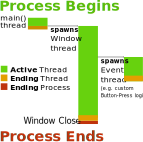
\includegraphics[width=0.95\textwidth]{Illustrations/ThreadExample_GUI}
		\label{fig:domains}
		\caption{Example GUI Program. \textbf{Three} threads are created within \textbf{one} process}
		\end{figure}
	\end{column}
\end{columns}

\end{frame}

\begin{frame}
\frametitle{Using Threads}

	\begin{itemize}
  		\item A \emph{multithreaded} program is a program that employs threads
  		
  		\linespace
  		
  		\item \emph{Concurrent} computing techniques are techniques that allow many tasks to occur at the same time [W]
  		
  		\linespace  		
  		
  		\item \emph{Parallel} computing techniques are techniques that allow many calculations to occur at the same time [W]
  		
  		\linespace  		
  		
  		\item Problems can be solved or improved using neither, either, or both of these techniques at once
	  \end{itemize}

\end{frame}


\begin{frame}
\frametitle{Using Threads}

One problem multithreaded programs face are called \emph{Race~Conditions}.

\linespace

Defined in Saltzer and Kaashoek as ``A timing-dependent error in thread coordination that may result in threads computing incorrect results.'' 

\linespace

Let's see an example where two threads increment a shared variable.
\end{frame}

\begin{frame}
\frametitle{Race Condition Example}
	\begin{figure}
		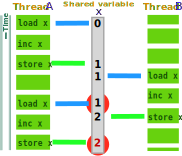
\includegraphics[width=0.8\textwidth]{Illustrations/RaceCondition}
		\label{fig:racecondition}
	\end{figure}

\end{frame}

\subsection[Locks]{Synchronicity and Locks}


\begin{frame}
\frametitle{Synchronicity and Locks}

\begin{itemize}
	\item Race conditions can be fixed by controlling access to shared data.
	\item This control is achieved by employing locks.
	
	\linespace
	
	\item \emph{Locks} secure objects or data shared between threads such that only one thread can read and write to it at one time.

	\linespace

	\item When a thread \emph{locks} a lock, that thread \textbf{acquires} the lock
	\item When a thread \emph{unlocks} a lock, that thread \textbf{releases} the lock
\end{itemize}

Now, let's fix the race condition in the previous example using locks

\end{frame}

\begin{frame}
\frametitle{Lock Example}
	\begin{figure}
		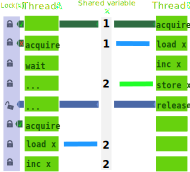
\includegraphics[width=0.8\textwidth]{Illustrations/Lock}
		\label{fig:lock}
	\end{figure}
\end{frame}

\section[Thread Scheduling]{Thread Scheduling on Linux}
\subsection[CFS]{Completely Fair Scheduler}
\begin{frame}
\frametitle{Completely Fair Scheduler (CFS)}

\begin{itemize}
\item Default Linux thread scheduler (there are others)
\item Handles which threads are executed at what times and on which CPU cores
\item Spend a \emph{fair} amount of runtime on all threads

\linespace

\item The scheduler \emph{switches} active threads on cores by saving and restoring thread and processor state information.
\item These switches are called \emph{context switches}.
\end{itemize}

We will continue to cover the CFS, then clarify process and thread state.
\end{frame}

\begin{frame}
\frametitle{Completely Fair Scheduler (CFS)}

\textbf{Goal:}
\begin{itemize}
\item Makes sure all threads run \emph{at least once} within arbitrary interval of CPU cycles
\item \emph{Timeslice} maximum cycles evenly amongst threads, factoring in thread weights\footnote{Priority (PR) and niceness (NI) values are responsible for determining process priority on Linux. We won't get into that here.}
\item The scheduler monitors the cycles that threads receive and switches them when they reach their max
\end{itemize}

\begin{figure}
		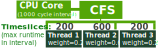
\includegraphics[width=0.8\textwidth]{Illustrations/CFS}
		\label{fig:cfs}
\end{figure}

\linespace

\end{frame}

\begin{frame}
\frametitle{Runqueues}

\begin{itemize}
	\item The data structure within CFS that contains threads is called a runqueue
	\item A \emph{runqueue} is a priority queue that sorts for threads that have received the least cycles in the current interval
	\item When a thread reaches its maximum time, the first thread in the runqueue is chosen	
\end{itemize}

\end{frame}


\begin{frame}
\frametitle{Runqueues on Multiple Cores}
If each core needs work to do, how do each of them receive threads?

\linespace

Will show that
\begin{itemize}
	\item If all cores shared one runqueue, cores would be doing frequent expensive book-keeping in order to search for available work and...
	\item Each core should have its own runqueue
\end{itemize}

\linespace

In order to understand the motivation for multiple runqueues, we need to know some about cache and processor state. (It will also help us later on)

\end{frame}



\subsection[Cache]{Thread State and Cache}
\begin{frame}
\end{frame}
\subsection[Load Balancing]{Load Balancing for CFS}
\begin{frame}
\end{frame}
\section[Bug Fixes and New Schedulers]{Bug fixes and two new schedulers}
\begin{frame}
\end{frame}

\section[Conclusions]{Conclusions}

\begin{frame}
\frametitle{Conclusions}

\begin{itemize}
  \item Added developmental plasticity to N-gram GP using Incremental Fitness-based Development (IFD).
\end{itemize}

\begin{itemize}
  \item IFD consistently improved N-gram GP performance on suite of test problems.
  
  \linespace
  
  \item ``Knocking out'' IFD shows it's valuable in all phases, even if it wasn't used earlier in a run.

  \linespace
  
  \item IFD generates more complex, less converged probability tables.
  \item IFD generates more modules/loops \& uses more low-probability paths.
\end{itemize}

\begin{itemize}
  \item Currently exploring applications to dynamic environments.
\end{itemize}

\end{frame}

\begin{frame}
\frametitle{Thanks!}

Thank you for your time and attention!
	
\linespace
\linespace

Contact:  
\begin{itemize}
	\item \texttt{mcphee@morris.umn.edu}
	\item \url{http://www.morris.umn.edu/~mcphee/}
\end{itemize}

\linespace
\linespace

\begin{center}
{\huge Questions?}
\end{center}
\end{frame}

\section*{References}

\begin{frame} 
\frametitle{References} 

\begin{thebibliography}{lskdjf}

\bibitem{Jo:2017}
H.~Jo, W.~Kang, C.~Min, and T.~Kim.

\newblock FLsched: A lockless and lightweight approach to OS scheduler for Xeon Phi.

\newblock In G\"unther Raidl, \emph{et al}, editors, {\em GECCO '09}, pages 1019--1026, Montr\'eal, Qu\'ebec, Canada, 2009.

\bibitem{Lozi:2016}
R.~Poli and N.~McPhee.
\newblock A linear estimation-of-distribution {GP} system.
\newblock In M.~O'Neill, \emph{et al}, editors, {\em EuroGP 2008}, volume
  4971 of {\em LNCS}, pages 206--217, Naples,
  26-28 Mar. 2008. Springer.
  
\end{thebibliography}

\linespace
\begin{center}
	See the GECCO '09 paper for additional references.
	\end{center}
\end{frame} 

\end{document}


